\FloatBarrier
\subsection{Review on the geometry of the observatory}\label{sec:georeview}
%\emph{Author(s): \textbf{Andreas Freise}, Stefan Hild} \\

This section briefly reviews the reasoning behind the shape of current gravitational wave detectors and then
discusses alternative geometries which can be of interest for third-generation detectors. We
will use the terminology introduced in the review of a triangular configuration~\cite{Freise2009} and
discriminate between the
\emph{geometry}, \emph{topology} and \emph{configuration} of a detector as follows:
\begin{itemize}
\item The \emph{geometry} describes the position information of one or several interferometers,
defined by the number of interferometers, their location and relative orientation.
\item The \emph{topology} describes the optical system formed by its core elements.
The most common examples are the Michelson, Sagnac and Mach--Zehnder topologies.
\item The \emph{configuration} describes the detail of the optical layout and the set of parameters that
can be changed for a given topology, ranging from the specifications of the optical core
elements to the control systems, including the operation point of the
main interferometer. Also the
addition of optical components to a given topology is often referred to as a change in configuration.
\end{itemize}

\FloatBarrier
\subsubsection{The L-shape}
\label{sec:lshape}
Current gravitational wave detectors represent the most precise instruments for measuring length changes.
They are laser interferometers with km-long arms and are operated differently from many precision
instruments built for measuring an absolute length. Viewed from above
they resemble an L-shape with equal arm length.
This geometric form follows directly from the nature of gravitational
waves: gravitational waves are transverse, quadrupole waves, thus a length change measured along any axis
occurs with opposite sign along the axis orthogonal to the previous one and the direction of propagation.
This key feature allows us to make a differential measurement between two orthogonal interferometer
arms, yielding twice the amplitude of a single arm. More importantly, a differential measurement allows us to
potentially discriminate between gravitational wave signals and those types of noise common to both arms, such as,
for example, laser amplitude noise. To achieve this the interferometer arms generally have to have approximately
the same length. The most simple L-shaped interferometer capable of doing this type
of measurement is the symmetric Michelson interferometer, on whose topology all current interferometric detectors
are based.

The long arm length of the detectors represents the simplest way to increase the signal-to-noise ratio
in the detector because for wavelength larger than the detector
dimensions, the `tidal' effect of the gravitational wave increases with the base length over which the
measurement is taken. In contrast the fundamental noises are connected to the interaction
of light with the optical components or the photo detection and thus do not scale with the length of the interferometer
arms.
We can summarise that for typical ground-based detectors with
sufficiently good vacuum and mirror position control systems, an increase in arm length will increase the
sensitivity of the detector proportionally.


Using the framework developed in~\cite{Jaranowski:1998qm} we can compute the sensitivity of a laser interferometer
with two arms to gravitational waves, taking into account the geometry of the detector, the location of the source and the
changes of both over time. The equations show directly that the arms of the detector do not
have to be perpendicular. A right angle, however, provides the maximum
response of an ideal detector to gravitational waves, which more generally can be written as
\begin{equation}
h(t)=F_{+}(t)h_{+}(t)+F_{\times}(t)h_{\times}(t)=\sin\zeta\,f(t,\psi, \dots)
\end{equation}
with $\zeta$ the opening angle of the interferometer arms, $F_{+}$ and $F_{\times}$ the beam pattern functions
and $f(t,\psi, \dots)$ a function of the remaining parameters describing the geometry (the location of the detector and
of the source in space and time and the wave polarisation angle).

In summary we can say that for a gravitational wave of given direction and polarisation, a properly aligned  symmetric L-shape
is an ideal optical layout for an interferometric
detector; the arms should be as long as possible and the sensitivity is maximised for an opening angle of $90^\circ$.
It should be noted that this does not put severe constraints on the type of interferometer topology used. In fact,
most common interferometer types can be used in a form that features two large symmetric arms in an L-shape
while potential other interferometer arms or sections are shortened such that they can be considered as part of one
corner of the detector.

\FloatBarrier
\begin{figure}[tbh]
\begin{center}
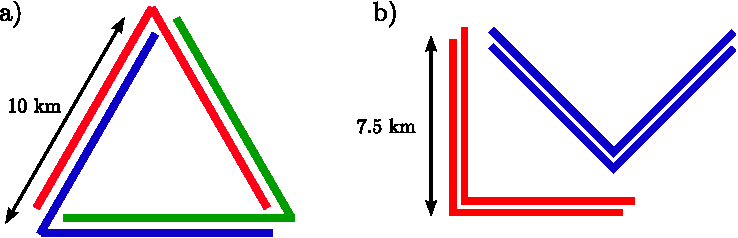
\includegraphics[width=0.7\textwidth,keepaspectratio]{Sec_Optics/TRIMI03}
\caption{{\bf a)} Triangle geometry: three L-shaped detectors with 10\, km arm length
are positioned in a equilateral triangle.
{\bf b)} Four L-shaped detectors at $0^\circ$ and $45^\circ$. The integrated length of all
interferometer arms in both configurations is 60\,km and two interferometer arms can share
the same structure. Note that for avoiding noise correlations between two detectors the
neighbouring interferometer arms would probably be housed in a separate vacuum tubes.}
\label{fig:triangle}
\end{center}
\end{figure}
\subsubsection{The triangle}
At any given moment an L-shaped detector can only detect one linear combination of polarisations of a
gravitational wave. However, for
estimation of source parameters from the measured signal, the full polarisation information is essential.
Thus it is of considerable interest to design a detector that is able to detect both polarisations (and thus the full content)
of a gravitational wave at all times. This can be achieved by combining two co-located
L-shaped detectors which are positioned at $45^\circ$ to each other. % (as shown in Figure~\ref{fig:triangle}).
More than 20 years ago it was recognised that a triangular geometry would provide the same
sensitivity to both polarisations as detectors at $45^\circ$ whilst requiring less enclosed space and fewer
end stations~\cite{Winkler1985}. In particular, the sensitivity of the two geometries shown
in Figure~\ref{fig:triangle} differs only by $6\%$~\cite{Freise2009}. The difference in the sensitivity to
different polarisations between a single L-shape and a triangular geometry can be best illustrated
with a plot of the so-called antenna pattern as shown in Figure~\ref{fig:triangleAP}.


\begin{figure}[t]
\begin{center}
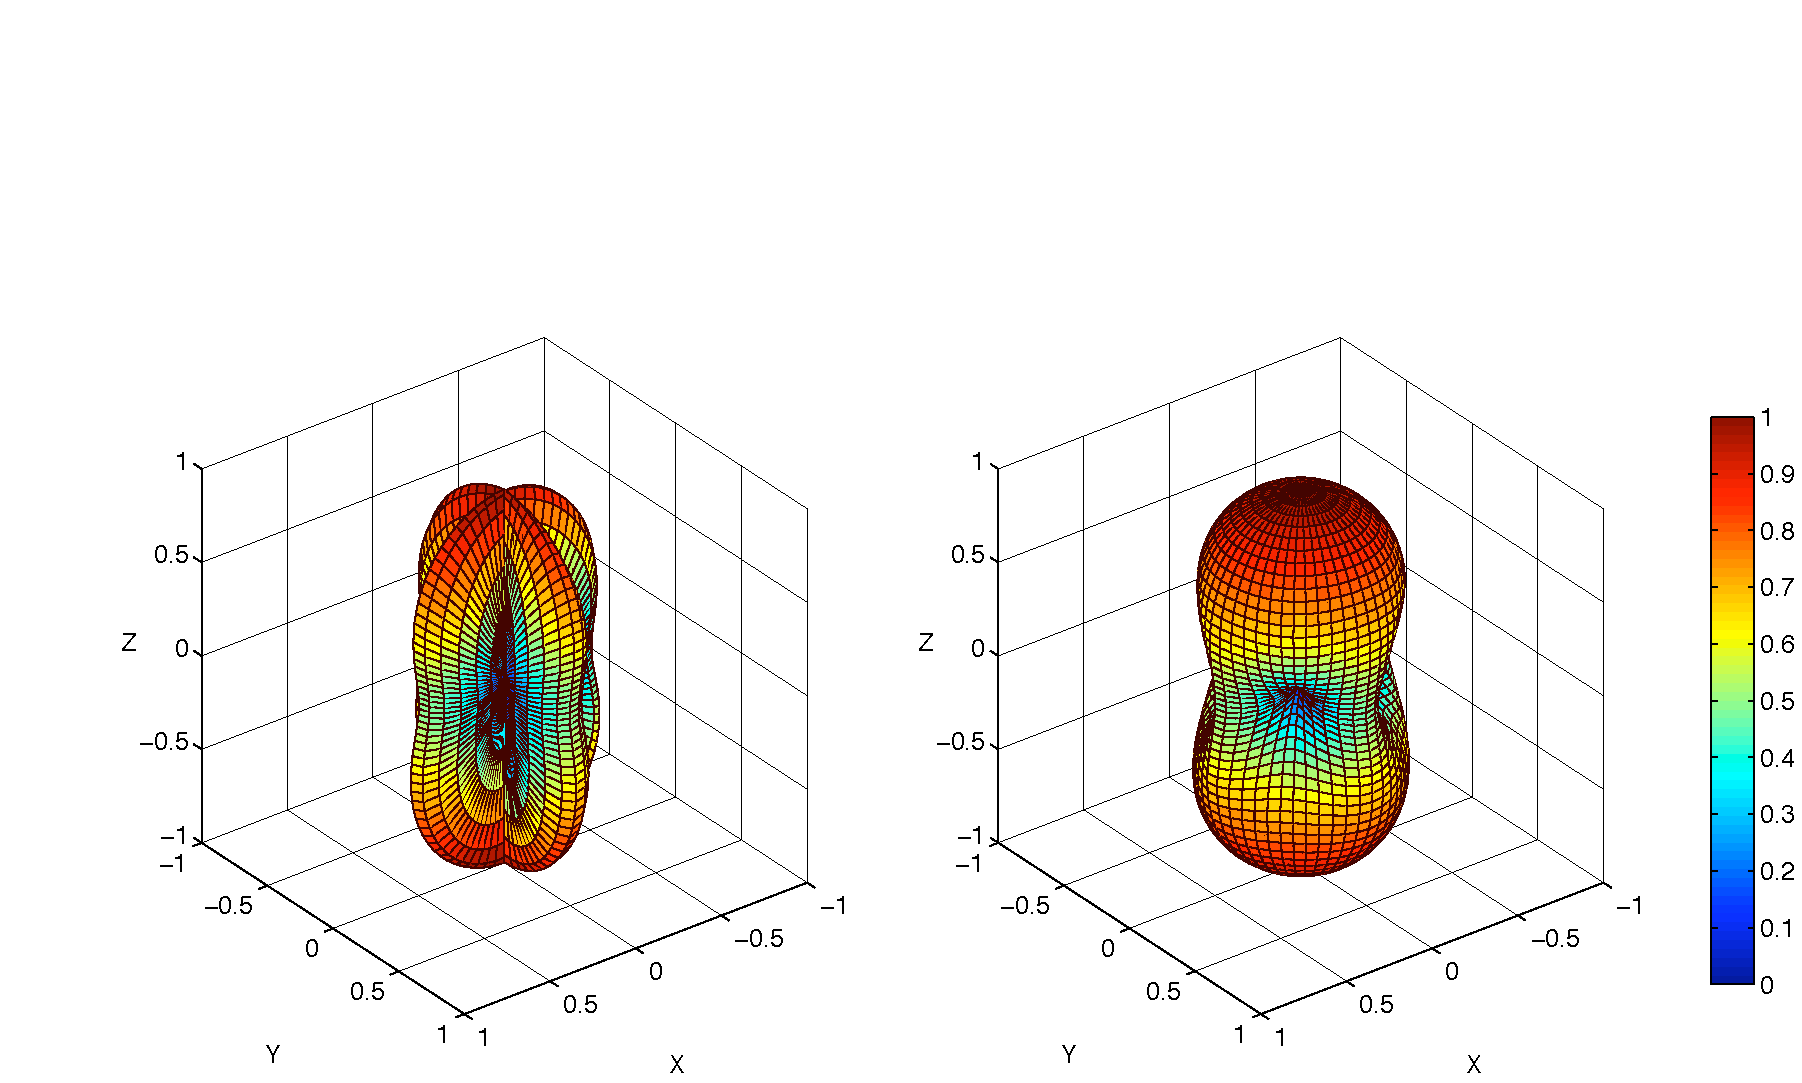
\includegraphics[width=0.9\textwidth, viewport= 50 0 885 370]{Sec_Optics/ap_mi_trimi.pdf}
\caption{The response of a detector to a linear polarised gravitational wave
as a function of the detector orientation. Both plots show the normalised sensitivity
to a wave travelling along the z-axis. Each data point represents the sensitivity of the
detector for a specific detector orientation defined by the detector normal
passing the respective data point and the origin. The colour
of the data point as well as its distance from the origin indicate the magnitude of the
sensitivity. The left plot depicts the response of a single Michelson, while the right plot
gives the response of a set of three interferometers in a  triangular geometry.
}
\label{fig:triangleAP}
\end{center}
\end{figure}
Using co-located detectors yields another advantage. Both layouts shown in Figure~\ref{fig:triangle} represent
detectors with redundancy. Redundancy here can be understood in relation to the continuous operation of the
detector as an observatory, or as a feature of the data streams generated by the full system. Redundancy in operation
is achieved by having multiple detectors which generate an equal or similar response to gravitational waves.
This is desirable in observatories which are expected to produce a quasi-continuous stream of astrophysically meaningful
data over a substantial amount of time. Typically laser interferometers cannot produce science data during
upgrades and maintenance work. Thus only alternating upgrades and data taking of redundant detectors can
avoid long down-times, for example during detector upgrades.

Such redundancy is obviously provided in the case of the 4 L-shaped  detectors, where two detectors are
always identical but can be operated independently. However, one can easily show that the triangular geometry
provides exactly the same redundancy~\cite{Freise2009}. For example, for three equal L-shaped interferometers
oriented at $0^\circ$, $120^\circ$ and $240^\circ$, one obtains:
\begin{equation}
-h_{0^\circ}= h_{240^\circ}+h_{120^\circ}\,,
\end{equation}
where the sign of the operation is defined by which ports of the interferometers
are used to inject the laser light. Thus the two interferometers at $120^\circ$ and $240^\circ$
create exactly the same response as the one at $0^\circ$. This allows
us to construct
so-called null-streams (or null-data streams)~\cite{GurselTinto1989}. Null-streams are a powerful
data analysis method that allows one to identify noise that is uncorrelated between the
detectors. Even though this does not increase the strain sensitivity of a detector,
it can add significantly to the robustness of the data processing
pipelines and thus to a larger number of detected events.
%lead, for example, to shorter delays between an event and the generation of a trigger for follow-up searches with optical telescopes.
The triangular geometry represents the minimal setup in one plane that can resolve both polarisations
and provides redundancy for the generation of null-streams.

\FloatBarrier
%\subsubsection{Interferometer Topologies }\label{sec:topologies}
To date no laser interferometer topology other than the Michelson has been
used for gravitational wave detection. However, some very advanced
noise reduction techniques proposed for future
detectors are based on topologies of the Sagnac interferometer, the Fox-Smith cavity or the
Mach-Zehnder interferometer~\cite{Chen2003,danilishin2006,Chen06b}.

It is worth noting that a triangular geometry as discussed above
is compatible with different interferometer
topologies. In particular it is possible to use different
topologies while maintaining the {\sf L}-shape of the single
interferometers
as displayed in figure~\ref{Fig:Lshape}.
Therefore, for example, three Sagnac interferometers or three cavities
could be used to form a triangle.
Such detector designs can provide similar benefits as described above for the
triple Michelson geometry so that the triangular geometry is largely independent
of the topology of the individual interferometers.

\longetbox{i}{ibox:topopt}{Different topology options}
{In this box we will list the different main interferometer
topologies that can be used for gravitational-wave detection and
describe their basic optical systems. A full gravitational-wave
detector could actually consist of more than one of those main
interferometers and could also be equipped with additional
techniques in order to achieve a specific susceptibility to the
quantum noise as will be described in Sec.~\ref{sec:qnr}.
Note that in principle, all of the mentioned interferometer
topologies can be fitted into
\begin{figure}[H]
\centering
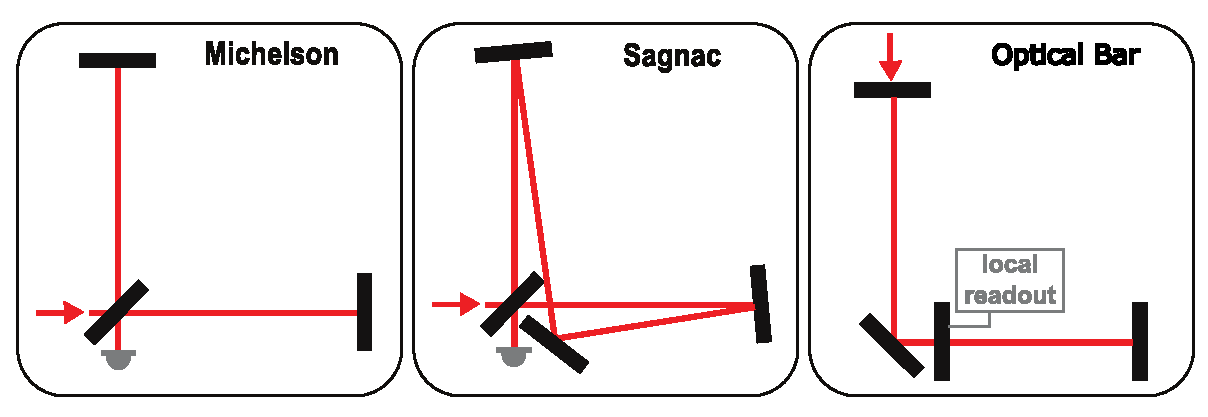
\includegraphics[width=15cm]{./Sec_Optics/Lshape.pdf}
\caption{Different (basic) topology options: simple Michelson
interferometer topology (left panel); zero-area Sagnac
interferometer topology (midd3le panel); optical bar topology
(right panel)
}\label{Fig:Lshape}
\end{figure}
an L-shape or into another two-arm shape under an arbitrary angle,
as shown in Fig.~\ref{Fig:Lshape}.
\begin{itemize}
\item {\bf Michelson interferometer} (basic): a laser beam is
split at a beam splitter and sent along two perpendicular
interferometer arms (cf.\ left panel of Fig.~\ref{Fig:Lshape}). The
ends of these arms (north and east) are marked by highly
reflective identical end mirrors, which reflect the beams back
into themselves so that they can be recombined at the beam
splitter. Generally, the Michelson interferometer has two outputs,
the south port and the west port (which is also the input port).
Both output ports can be used to obtain interferometer signals,
however, most setups are designed in such a way that the signals
are detected at the south port. For the detection of gravitational
waves, the Michelson interferometer has to be sensitive to small
perturbations in the difference of the two arm lengths and the
phase relation is chosen in such a way that this signal interferes
constructively at the south port.
Usually the south port is kept
nearly dark, with all light reflected back to the west input port,
then also called the bright port of the interferometer. A
power-recycling mirror can be positioned at the bright port in
such a way that it forms a resonant cavity for the carrier light
together with the mirrors of the two interferometer arms.
Furthermore, each interferometer arm can be replaced by equal
Fabry-Perot cavities, formed by an input mirror and an
end mirror. An additional mirror can also be placed at the
interferometer's south port, known as the signal-recycling mirror.
Another possibility is to send the output signal at the west port
into an additional resonator, a so-called sloshing cavity.
Furthermore, polarizing optics can be used in order to send the
beam back into the interferometer. The Michelson interferometer is
the standard topology for interferometric gravitational-wave
detectors. The great advantage of this configuration is that there is a lot of
experience gathered.
\item  {\bf Sagnac interferometer} (basic): a laser beam is split
into two beams at the beam splitter which both travel through the
whole interferometer but in opposite directions. The two beams are
recombined at the beam splitter. The interferometer has only one
output port, namely the south port. A Sagnac
interferometer is by construction always operated at a dark port, i.e.
all carrier light is reflected back to the input port. The
arms can be folded in such a way that both beams circulate around
a zero area (cf.\ middle panel of Fig.~\ref{Fig:Lshape}) in order
to make the interferometer insensitive to rotations and forming
two perpendicular interferometer arms. Those arms can be replaced
by ring resonators, either of rectangular or triangular shape. For
the Sagnac interferometer topology, an additional mirror at the
input port can realize power-recycling and an additional mirror
at the output port can realize signal-recycling. Up to now a
Sagnac interferometer has never been adopted as a large-scale
interferometric gravitational-wave detector. Only some features
have been tested in table-top experiments and a theoretical study
has started to explore noise couplings in a Sagnac
interferometer~\cite{Chelkowski}.
\item {\bf Optical bar}: The optical bar topology is an optical
realization of a mechanical resonant bar gravitational-wave
detector. It essentially consists of two coupled optical
resonators, which are shaped as a L and coupled through a light,
partially transmissive mirror as shown in the right panel of
Fig.~\ref{Fig:Lshape}. An additional local meter is applied to the
central mirror, reading out its motion. The local meter could in
principle be any device but its sensitivity is essentially
determining the sensitivity of the optical bar detector. It is
even not obligatory for the local meter to be an optical device,
for instance it could be a SQUID-based microwave meter as a speed
meter, or some other high precision superconductive sensor. The
optical bar topology can be transformed into an optical lever
topology by inserting an additional mirror into each arm of the L,
forming a resonant cavity together with the corresponding end
mirror.
\end{itemize}}

The case for alternative topologies is largely based on ideas for the
reduction of quantum noise. In general, the signal-to-noise ratio of a
single interferometer is different for each topology, with the actual
difference depending also on the type of noise under investigation.
However, it is not possible to identify a topology with a meaningful
signal-to-noise ratio or sensitivity since these vary dramatically
with the interferometer \emph{configuration}.

During the design and construction of the first generation of detectors
the Sagnac topology has been investigated and prototypes have been
built~\cite{Sun1996} but it did not show significant advantages over the Michelson
topology~\cite{Mizuno97}. More recently it has been proposed to use the Sagnac topology
as a \emph{speed meter}~\cite{Chen2003} to reduce the quantum noise.
The Sagnac topology can be hosted in different ways in a triangular
geometry: each Sagnac as an equilateral triangle, or as an {\sf L}-shaped
zero-area Sagnac. Noise couplings due to the Sagnac effect favor the
zero-area Sagnac topology: it can be shown that for a typical
choice of optical parameters the extra noise couplings do not
impose stringent new requirements in the case of a zero-area Sagnac
interferometer \cite{Freise2009}.

We note that Michelson-based detectors currently offer the
advantage of using the experience as well as the
advanced optical technologies of the first two detector generations.




%%
%The geometry of an observatory is determined by the number of%
%detectors, their location and relative%
%orientation~\cite{Freise2009}. Short review of ET in a world wide%
%network:%
%\begin{itemize}%
%\item we assume ET to be part of such a network and thus only%
%consider the optical layout of one site%
%\item in first order the%
%optical layout is then independent of the details of%
%  the network%
%\end{itemize}%
%Reasoning for single site… For the ET detector we propose an%
%infrastructure (cf. Sec.~???) for three detectors, where the arms%
%are aligned in such a way that together they form an equilateral%
%triangle as shown in Fig.~???. Reasoning for three detectors…%
%Each of the three detectors can consist of different co-located%
%sub-system interferometers, which for example take care about%
%different frequency bands (cf. Sec.~\ref{sec:toporeview}). Discuss%
%geometry issues: sky position, resolution, gravitational-wave%
%polarization… or refer to Sec.~???.%
%%
%In the following we will almost always describe the features of%
%only one of this three detectors.%
